\documentclass[11pt,a4paper]{article}
\usepackage[margin=2.2cm]{geometry}
\usepackage{fontspec}
\setmainfont{Segoe UI}[BoldFont={Segoe UI Bold}]
\setmonofont{Consolas}[Scale=0.92]
\newfontfamily\thai{Tahoma}
\usepackage{xcolor}
\definecolor{accent}{HTML}{4F46E5}
\definecolor{muted}{HTML}{6B7280}
\definecolor{soft}{HTML}{EEF2FF}
\definecolor{warn}{HTML}{FEF3C7}
\definecolor{blue}{HTML}{3B82F6}
\definecolor{green}{HTML}{22C55E}
\definecolor{amber}{HTML}{F59E0B}
\definecolor{rose}{HTML}{F43F5E}
\definecolor{purple}{HTML}{A855F7}
\definecolor{orange}{HTML}{F97316}
\usepackage{tikz}
\usetikzlibrary{positioning,arrows.meta,fit,shapes.misc}
\usepackage{booktabs,tabularx,array}
\usepackage{enumitem}
\setlist{itemsep=2pt,topsep=4pt}
\usepackage{titlesec}
\titleformat{\section}{\Large\bfseries\color{accent}}{\thesection}{0.6em}{}
\titleformat{\subsection}{\large\bfseries}{\thesubsection}{0.6em}{}
\titlespacing*{\section}{0pt}{18pt}{8pt}
\usepackage{fancyhdr}
\pagestyle{fancy}\fancyhf{}
\fancyhead[L]{\small\color{muted}Thotsakan Statistics — guide to the documentation}
\fancyhead[R]{\small\color{muted}27 October 2026}
\fancyfoot[C]{\small\color{muted}\thepage}
\renewcommand{\headrulewidth}{0.3pt}
\usepackage[skins,breakable]{tcolorbox}
\newtcolorbox{note}[1][]{colback=soft,colframe=accent,boxrule=0.5pt,arc=2pt,left=8pt,right=8pt,top=6pt,bottom=6pt,breakable,#1}
\newtcolorbox{rulebox}[1][]{colback=warn,colframe=amber,boxrule=0.5pt,arc=2pt,left=8pt,right=8pt,top=6pt,bottom=6pt,breakable,#1}
\usepackage[hidelinks]{hyperref}
\newcommand{\f}[1]{\texttt{#1}}
\setlength{\parindent}{0pt}
\setlength{\parskip}{6pt}
\renewcommand{\arraystretch}{1.25}
\newcolumntype{L}{>{\raggedright\arraybackslash}X}

\begin{document}

\begin{titlepage}
\vspace*{3cm}
{\color{accent}\Huge\bfseries Thotsakan Statistics\par}
\vspace{4pt}
{\Large{\thai ทศกัณฐ์ สถิติ}\par}
\vspace{18pt}
{\LARGE A guide to the documentation\par}
\vspace{10pt}
{\large\color{muted} What each document says, how the app is built, and how to work on it\par}
\vspace{2.5cm}
\begin{note}
\textbf{For:} Irving Gomez (lab head) and the students who work on the project.\\[3pt]
\textbf{Describes:} the code and documents on branch \f{irving-reviewing-experiment}, 27 October 2026,
a week before v1 is deployed (Wednesday 4 November 2026).\\[3pt]
\textbf{How to use it:} this guide is a map. The documents in the repository are the source of truth; when
they change, they win over this PDF.
\end{note}
\vfill
{\color{muted}\small Contents: 1 The app in one page · 2 The documents · 3 Decisions and rules · 4 Architecture ·
5 Inside a tab · 6 Working on the project · 7 Status and what comes next · 8 Glossary\par}
\end{titlepage}

% ------------------------------------------------------------------
\section{The app in one page}

Thotsakan Statistics is a web \textbf{statistics analysis tool} for CMKL students and staff, in the style of
jamovi or JASP. You load a dataset, pick a variable and the options you want, and the tables, plots and
formulas update by themselves. The app reports numbers and draws plots; \textbf{the user decides}. It never
prints a verdict such as ``Reject H\textsubscript{0}'', and it has no lessons or teaching flow.

The name comes from the giant Thotsakan, who has ten faces and twenty arms to see and control the world from
every angle: the app gives its users ``ten arms'' (sliders, switches, selectors) to change the variables and
watch the data respond.

\begin{center}
\begin{tabularx}{\textwidth}{@{}lL@{}}
\toprule
\textbf{Tab} & \textbf{What it does} \\
\midrule
Home & Welcome page. \\
Data & Upload a comma-separated CSV file, or open one of three example datasets (World Happiness Report 2023 — the default, Howell, Victoria electricity demand 2014). Fix column types, filter categories, set display precision. \\
Probability › Common Distributions & PMF/PDF of 12 distributions, with the area of a query such as P(X ≤ 5) or P(2 < X ≤ 5). \\
Statistics › Graphical Analysis & Histogram or ECDF of a variable, with KDE, a normal model and a confidence band. \\
Statistics › Descriptive Statistics & Quantiles, centre, spread and shape, with estimator tags (Unbiased / Consistent); histogram and box plot. \\
Statistics › Statistical Inference & Confidence and prediction intervals (normal theory and bootstrap); confidence regions for (μ, σ). \\
Hypothesis Testing & One- and two-sample t, Bartlett / Levene, one-way ANOVA; α, critical values, rejection region. Works, but needs a deep rework after v1. \\
Linear Regression & Planned. \\
\bottomrule
\end{tabularx}
\end{center}

\textbf{v1} is the version deployed on 4 November 2026 and shown at the event on 6 November. It covers the
Data tab and the four tabs Common Distributions, Graphical, Descriptive and Inference, all made consistent with
each other. Hypothesis Testing stays as it is; Linear Regression and other file formats come later.

% ------------------------------------------------------------------
\section{The documents: what each file holds}

All documentation lives in the folder \f{docs/}, plus a few files at the top of the repository. Read them in
the order of the first column when you join the project.

\begin{center}
\begin{tabularx}{\textwidth}{@{}c>{\raggedright\arraybackslash}p{4.75cm}L@{}}
\toprule
\textbf{Read} & \textbf{File} & \textbf{What it holds — and when to open it} \\
\midrule
1 & \f{README.md} & The front page: what the app does, the feature table, how to install and run it, how to run the tests, and the list of documents. \emph{Open first.} \\
2 & \f{docs/decisions.md} & Every decision on how the app looks and behaves, dated, taken by Irving Gomez, with the commits that built it and, where recorded, the reason. \emph{Open before changing anything visible.} \\
3 & \f{docs/interaction\_}\newline\f{contract.md} & The 17 rules every analysis tab follows (options, automatic results, tables and plots, naming, layout, colors). \emph{Open when you build or change a tab.} \\
4 & \f{docs/design.md} & What the app is, the three panels, the DualInput control, the theme and the performance budget. Also the long-term idea of a guided-teaching layer (not built). \\
5 & \f{docs/architecture.md} & How the frontend and backend fit together: layers, folders, request flow, sessions, filters, every API endpoint, testing and CI. \emph{Open when you write code.} \\
6 & \f{docs/roadmap.md} & The authoritative feature status, the one backlog after v1 (in priority order), the Linear Regression plan, migration notes and the open known issues. \emph{Open when you look for work.} \\
— & \f{docs/AUTH.md} & How to set up Google sign-in (restricted to \f{@cmkl.ac.th}) and fix sign-in problems. \\
— & \f{docs/plans/}\newline\f{2026-10-23-v1-release.md} & The checklist of the steps to v1 (A done, B done, C documentation, D release, E protection). Removed after the deploy. \\
— & \f{CONTRIBUTING.md} & Workflow, coding standards, how to test, how to write commits and pull requests. \\
— & \f{AGENT.md} & Instructions for AI coding assistants (Claude Code, Codex, …): the same rules, written for them. Will be renamed \f{AGENTS.md}. \\
— & \f{CODE\_OF\_CONDUCT.md} & How we treat each other. \\
— & \f{changelogs/} & One dated note per batch of changes: what changed, in plain words. \\
\bottomrule
\end{tabularx}
\end{center}

\begin{note}
\textbf{One fact, one place.} Each kind of information has exactly one home: decisions in
\f{decisions.md}, rules in the contract, feature status and backlog in \f{roadmap.md}, how the code works in
\f{architecture.md}. Other documents link there instead of repeating it, so nothing goes out of date twice.
\end{note}

% ------------------------------------------------------------------
\section{Decisions and rules: what nobody changes alone}

\begin{rulebox}
\textbf{The rule.} Nobody — student or AI agent — reverses or works around a decision recorded in
\f{docs/decisions.md}. If the change you want conflicts with one, stop and talk to Irving first. A decision
changes only through a new dated entry in that file, written or approved by Irving. The interaction contract
changes the same way: ask Irving, record the decision, change the contract, then the code.
\end{rulebox}

\subsection*{The decisions that shape everything}
\begin{itemize}
\item \textbf{An analysis tool, not a guided lab.} The app reports; the user decides. No verdicts, no lessons.
\item \textbf{Results update on their own.} About 250 ms after a change (700 ms while bootstrap is on). No Run
  button, only Reset — and Reset shows the result for the defaults straight away.
\item \textbf{Three panels, always the same order.} Left: inputs only (what to show first, then one Settings
  section). Center: tables at the top, plots below. Right: the formulas of what is on screen, then a closing
  ``Values'' section.
\item \textbf{Formulas are copied from the code} in \f{backend/core/}, never from a textbook, and only for what
  was chosen.
\item \textbf{One meaning per color.} In every plot: mean {\color{blue}\textbf{blue}}, median
  {\color{green}\textbf{green}}, deviation {\color{amber}\textbf{amber}}, prediction {\color{rose}\textbf{rose}},
  KDE {\color{purple}\textbf{purple}}, normal model {\color{orange}\textbf{orange}}. All colors live in
  \f{frontend/src/plot/theme.ts}.
\item \textbf{Readable text.} Small text is 14 px; nothing, plots included, is under 12 px.
\item \textbf{Data.} CSV only for now. A column is numeric when at least 80\% of its filled cells are numbers;
  the other cells count as missing. Filters compare values as written in the CSV.
\end{itemize}
The full list (29 entries) with dates and commits is in \f{docs/decisions.md}.

\subsection*{The contract in five lines}
\begin{enumerate}
\item \textbf{Options:} a hidden option is never sent; show an option only when it applies; never force an
  input; sensible defaults ticked; options that only change the display never recalculate.
\item \textbf{Running:} automatic, debounced; one shared status component for computing, errors and warnings.
\item \textbf{Results:} adding a method adds rows (bootstrap next to normal theory); the program reports, the
  user decides; warnings only where they apply.
\item \textbf{Naming:} one display-name map (\f{labels.ts}); α is always ``Significance level α''; discrete
  probabilities are bars.
\item \textbf{Layout and states:} shared components and shared colors, never per-tab copies.
\end{enumerate}


\newpage
\section{Architecture}

The app has two halves. The \textbf{frontend} (React, in \f{frontend/}) draws the screen. The \textbf{backend}
(FastAPI in Python, in \f{backend/}) does every statistical calculation. The professor checks the mathematics
by reading \f{backend/core/}.

\begin{center}
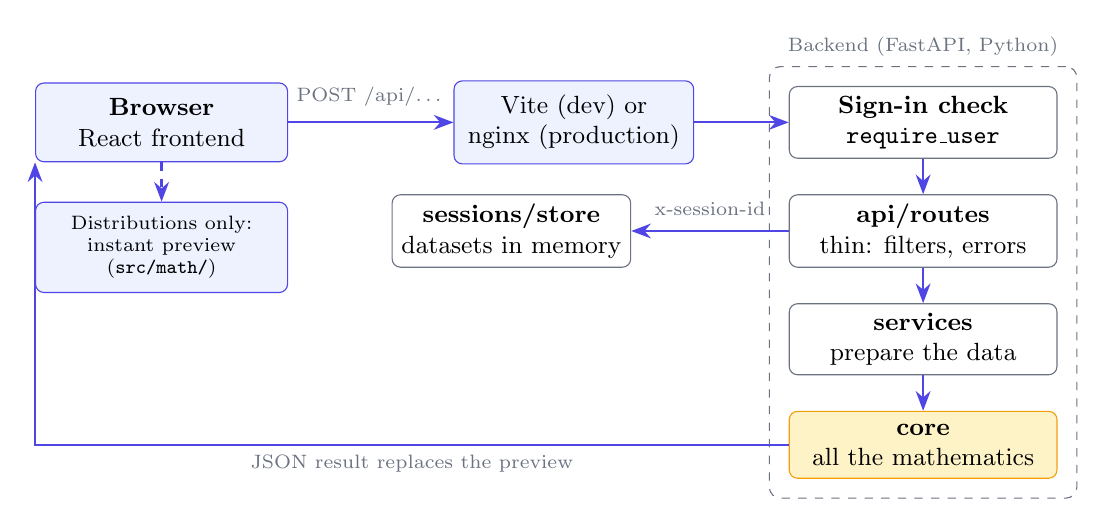
\begin{tikzpicture}[
  box/.style={draw=accent,fill=soft,rounded corners=3pt,align=center,minimum height=1cm,font=\small,inner sep=5pt},
  lay/.style={draw=muted,fill=white,rounded corners=3pt,align=center,minimum width=3.4cm,minimum height=0.85cm,font=\small},
  arr/.style={-{Stealth[length=2.5mm]},thick,color=accent},
  lbl/.style={font=\scriptsize,color=muted,align=center}]
\node[box,minimum width=3.2cm] (browser) {\textbf{Browser}\\React frontend};
\node[box,below=0.5cm of browser,minimum width=3.2cm,font=\scriptsize] (preview) {Distributions only:\\instant preview\\(\f{src/math/})};
\node[box,right=2.1cm of browser,minimum width=2.6cm] (proxy) {Vite (dev) or\\nginx (production)};
\node[lay,right=1.2cm of proxy] (auth) {\textbf{Sign-in check}\\\f{require\_user}};
\node[lay,below=0.45cm of auth] (routes) {\textbf{api/routes}\\thin: filters, errors};
\node[lay,below=0.45cm of routes] (services) {\textbf{services}\\prepare the data};
\node[lay,below=0.45cm of services,fill=warn,draw=amber] (core) {\textbf{core}\\all the mathematics};
\node[lay,left=2.0cm of routes,minimum width=2.6cm] (store) {\textbf{sessions/store}\\datasets in memory};
\node[draw=muted,dashed,rounded corners=4pt,inner sep=7pt,fit=(auth)(routes)(services)(core),label={[lbl]above:Backend (FastAPI, Python)}] {};
\draw[arr] (browser) -- node[lbl,above=2pt]{POST /api/…} (proxy);
\draw[arr] (proxy) -- (auth);
\draw[arr] (auth) -- (routes);
\draw[arr] (routes) -- (services);
\draw[arr] (services) -- (core);
\draw[arr] (routes) -- node[lbl,above=2pt]{x-session-id} (store);
\draw[arr,dashed] (browser) -- (preview);
\draw[arr] (core.west) -| node[lbl,pos=0.25,below]{JSON result replaces the preview} (browser.south west);
\end{tikzpicture}
\end{center}

\subsection{What happens when you move a slider}
\begin{enumerate}
\item You change a setting in the left panel. The tab's state hook waits about 250 ms for you to stop.
\item In Common Distributions only, the browser first draws an instant \emph{preview} with its own copy of the
  formulas (\f{frontend/src/math/}). It must give the same numbers as the backend.
\item The hook cancels any older request still on its way and sends a new one (\f{POST /api/…}) with the
  dataset's session id in the \f{x-session-id} header.
\item The backend checks you are signed in, finds your dataset in memory, applies the Data tab's filters, and
  calls the service, which prepares the data and calls \f{core/}.
\item \f{core/} computes at full precision; the result comes back as JSON and is drawn. Rounding happens only
  on screen.
\end{enumerate}

\subsection{The backend in layers}
Each layer may only call the layer below it. This keeps the mathematics in one place the professor can check.
\begin{center}
\begin{tabularx}{\textwidth}{@{}>{\raggedright\arraybackslash}p{3.3cm}L@{}}
\toprule
\textbf{Folder} & \textbf{Job and rules} \\
\midrule
\f{api/routes/} & One file per area. Thin: apply the filters, call the service, turn a \f{ValueError} into a 400 error. Every router gets its URL prefix in \f{main.py}. \\
\f{api/schemas/} & The shape of each request and response (Pydantic models). \\
\f{api/deps.py} & Shared helpers: the sign-in check, finding the dataset (\f{get\_session\_data}), and the one filter every tab uses (\f{apply\_filters}). \\
\f{services/} & Prepare the data (missing values, weights) and map results to schemas. May \emph{not} import numpy, scipy or statsmodels. \\
\f{core/} & All mathematics, at full precision. Imports nothing from the rest of the project. Files copied from the professor's original app are kept byte-identical; new behaviour goes in new files next to them. \\
\f{sessions/store.py} & Uploaded datasets in memory, 30 minutes after last use; a restart clears them. That is why the backend runs a single worker. \\
\bottomrule
\end{tabularx}
\end{center}

\subsection{The frontend folders}
\begin{center}
\begin{tabularx}{\textwidth}{@{}>{\raggedright\arraybackslash}p{3.3cm}L@{}}
\toprule
\textbf{Folder} & \textbf{What is inside} \\
\midrule
\f{features/} & One folder per tab (\f{data/}, \f{probability/common/}, \f{estimation/graphical/}, \f{estimation/descriptive/}, \f{estimation/inference/}, \f{hypothesis/}). \\
\f{components/} & Shared pieces every tab uses: \f{StatusBanner}, \f{ResultTable}, \f{ResultSection}, \f{CheckboxTree}, \f{MathFormula} (KaTeX), \f{DualInput}, form controls, export menu. \\
\f{plot/theme.ts} & Every plot color and the shared Plotly look. \\
\f{labels.ts} & One display name for every statistic and estimator. \\
\f{api/} & One small file per backend area, with the request and response types. \\
\f{context/} & \f{DataContext} (the dataset, its session id, column types, filters) and \f{AuthContext} (sign-in). \\
\f{layout/} & The page frame: logo bar, header, sub-header, the three-panel \f{LabBench}, footer. \\
\f{math/} & The distributions preview only. No other statistics in the frontend. \\
\bottomrule
\end{tabularx}
\end{center}

\subsection{Datasets, sign-in and filters}
\begin{itemize}
\item \textbf{Sign-in:} Google, restricted to verified \f{@cmkl.ac.th} accounts; the backend sets a signed
  cookie. Setup in \f{docs/AUTH.md}.
\item \textbf{Datasets:} the Data tab reads the CSV in the browser (for the preview and the filter lists) and
  also uploads it. The backend keeps it in memory under a session id, which the frontend sends with every
  analysis request. Both sides use the same 80\% rule to decide which columns are numbers.
\item \textbf{Filters:} chosen in the Data tab, sent with each request and applied on the server by one shared
  function, so every tab analyses exactly the same rows.
\end{itemize}

\subsection{The API at a glance}
\begin{center}
\small
\begin{tabularx}{\textwidth}{@{}>{\raggedright\arraybackslash}p{5.2cm}L@{}}
\toprule
\textbf{Endpoint} & \textbf{Purpose} \\
\midrule
\f{GET /api/health} & Is the backend alive? \\
\f{/api/auth/…} & Sign-in configuration, Google sign-in, current user, sign-out. \\
\f{POST /api/data/upload} & Upload a CSV; returns the dataset's session id and column types. \\
\f{POST /api/probability/compute} & One distribution: PMF/PDF, the query's probability, mean and variance. \\
\f{POST /api/descriptive/compute} & Descriptive statistics, histogram and box plot data. \\
\f{POST /api/inference/estimators} & Which estimators suit a column. \\
\f{POST /api/inference/ci}, \f{/pi}, \f{/regions} & Confidence intervals, prediction intervals, confidence regions. \\
\f{POST /api/graphical/compute} & Histogram or ECDF with its overlays. \\
\f{POST /api/hypothesis/test} & One of four tests with α, critical values and rejection region. \\
\bottomrule
\end{tabularx}
\end{center}

% ------------------------------------------------------------------
\section{Inside a tab}

Every analysis tab is built the same way, so once you know one you know them all.

\begin{center}
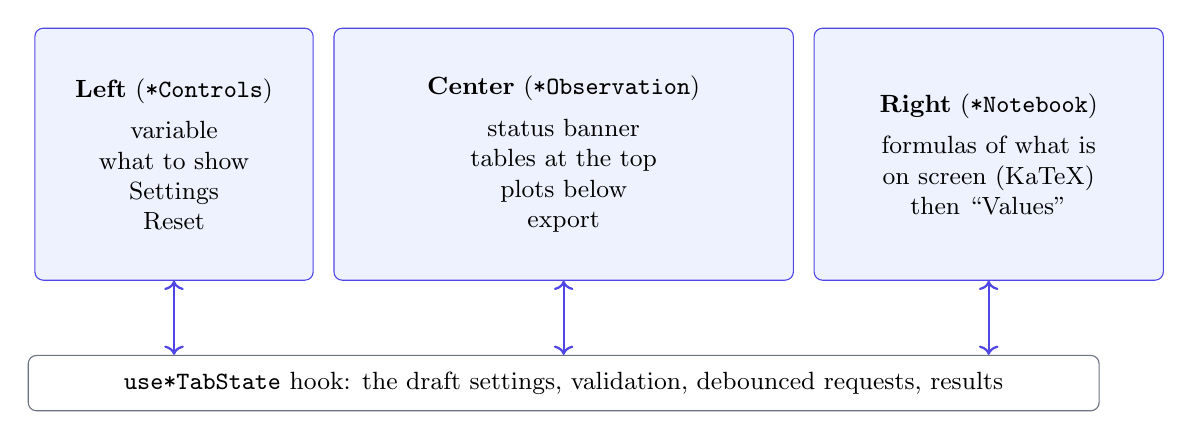
\begin{tikzpicture}[
  p/.style={draw=accent,fill=soft,rounded corners=3pt,minimum height=3.2cm,align=center,font=\small,text width=#1},
  arr/.style={-{Stealth[length=2.5mm]},thick,color=accent}]
\node[p=3.3cm] (l) {\textbf{Left} (\f{*Controls})\\[4pt]variable\\what to show\\Settings\\Reset};
\node[p=5.6cm,right=0.25cm of l] (c) {\textbf{Center} (\f{*Observation})\\[4pt]status banner\\tables at the top\\plots below\\export};
\node[p=4.2cm,right=0.25cm of c] (r) {\textbf{Right} (\f{*Notebook})\\[4pt]formulas of what is\\on screen (KaTeX)\\then ``Values''};
\node[draw=muted,rounded corners=3pt,fill=white,align=center,font=\small,inner sep=6pt,
  minimum width=13.6cm] (h) at ([yshift=-1.3cm]c.south) {\textbf{\f{use*TabState}} hook: the draft settings, validation, debounced requests, results};
\draw[arr,<->] (l.south) -- (l.south |- h.north);
\draw[arr,<->] (c.south) -- (c.south |- h.north);
\draw[arr,<->] (r.south) -- (r.south |- h.north);
\end{tikzpicture}
\end{center}

\begin{itemize}
\item The three panels are exported from one \f{*Tab.tsx} file and placed into the shared \f{LabBench} layout
  by \f{App.tsx}. The layout never changes; a tab only fills the three slots.
\item The \f{use*TabState} hook is created in \f{App.tsx}, so a tab keeps its settings when you switch away.
\item Separate \emph{request} settings (they change the calculation) from \emph{display} settings (they only
  change what is shown and never recalculate).
\item Use the shared components and \f{plot/theme.ts}; do not write a per-tab status box, table style or
  color.
\end{itemize}

% ------------------------------------------------------------------
\section{Working on the project}

\subsection{Run it}
\begin{tabularx}{\textwidth}{@{}>{\raggedright\arraybackslash}p{7.6cm}L@{}}
\toprule
\textbf{Command (from the repository root)} & \textbf{Gives you} \\
\midrule
\f{docker compose -f docker-compose.dev.yml up} & Development stack with hot reload: app on \f{localhost:5173}. \\
\f{docker compose up --build} & Production-style stack: app on \f{localhost:8080}. \\
\f{npm install \&\& npm run dev} & Without Docker: frontend on :5173, backend on :8000. \\
\bottomrule
\end{tabularx}

The backend refuses to start until sign-in is configured in the root \f{.env} file (see \f{docs/AUTH.md}); on
your own machine you may set \f{AUTH\_DISABLED=true} instead.

\subsection{Test it — before every commit}
\begin{tabularx}{\textwidth}{@{}>{\raggedright\arraybackslash}p{6.4cm}L@{}}
\toprule
\f{cd backend \&\& pytest} & Backend tests (about 220). \\
\f{cd frontend \&\& npm run test} & Frontend tests (about 250). \\
\f{cd frontend \&\& npm run build} & Type check and production build. \\
\bottomrule
\end{tabularx}

The continuous-integration workflow does not run the tests yet (it is planned), so run them yourself and report
the real result.

\subsection{Change it}
\begin{enumerate}
\item Read \f{decisions.md} and the interaction contract. If your idea conflicts with either, talk to Irving
  first.
\item Write a test that shows the problem or the new behaviour; see it fail.
\item Make the change in the right layer: mathematics in \f{core/}, data preparation in \f{services/},
  screens in \f{features/}, shared look in \f{components/} and \f{plot/theme.ts}.
\item Run the three test commands above.
\item Update the documents the change touches: the feature table in \f{roadmap.md} and \f{README.md}, a dated
  note in \f{changelogs/}, and \f{decisions.md} if Irving took a new decision.
\item Commit with a Conventional Commit message (\f{feat:}, \f{fix:}, \f{docs:}, …) and open a pull request.
\end{enumerate}

\begin{note}
\textbf{Never:} add statistics to the frontend; edit the professor's original files in \f{core/}; invent
reference values for tests (check them against scipy, statsmodels or a cited source); commit a real dataset or
a secret; add a dependency without approval.
\end{note}

% ------------------------------------------------------------------
\section{Status and what comes next}

\subsection{Steps to v1}
\begin{tabularx}{\textwidth}{@{}lL@{}}
\toprule
\textbf{Step} & \textbf{State on 27 October 2026} \\
\midrule
A. Consistency additions & Done (intervals table, formulas, colors, plotting rules). \\
B. Correctness and review & Done (weights bug, final review of the branch). \\
C. Documentation & C1 \f{docs/} rename, C2 decision log, C3 documents updated: done. C4 one version number (1.0.0, semantic versioning): done. \\
D. Release & Full verification, merge into \f{dev}, deploy on Wednesday 4 November. \\
E. Protecting the decisions & Right after the merge: \f{AGENTS.md}, tests in CI, branch protection on GitHub. \\
\bottomrule
\end{tabularx}

\subsection{After v1}
The backlog in \f{docs/roadmap.md}; the first three in the order Irving set:
\begin{enumerate}
\item A goodness-of-fit test for the normal distribution, shown at the top of the left panel wherever a result
  assumes normal data.
\item A deep rework of Hypothesis Testing.
\item Linear Regression.
\item Classifying variables (continuous, discrete, ordinal, nominal, …) instead of guessing from the values.
\item Data tab: Excel and SPSS files; better handling of very large datasets.
\item Backend tidy-up, small interface items, and later the custom distributions, approximations, Thai /
  English text and the guided-teaching layer.
\end{enumerate}

% ------------------------------------------------------------------
\section{Glossary}
\begin{tabularx}{\textwidth}{@{}>{\raggedright\arraybackslash}p{3.6cm}L@{}}
\toprule
Backend / frontend & The Python server that computes / the React web page that shows. \\
Session id & The key under which the backend keeps your uploaded dataset in memory. \\
Debounce & Waiting a short moment after the last change before sending a request, so a burst of changes becomes one request. \\
Provisional preview & The instant curve drawn by the browser in Common Distributions, replaced by the backend's result. \\
Request vs display setting & One that changes the calculation vs one that only changes what is shown. \\
Interaction contract & The 17 rules every analysis tab follows (\f{docs/interaction\_contract.md}). \\
Decision log & The dated list of Irving's decisions (\f{docs/decisions.md}). \\
Conventional Commits & Commit messages that start with a type: \f{feat:}, \f{fix:}, \f{docs:}, \f{refactor:}. \\
CI & Continuous integration: the GitHub workflow that builds the app when \f{dev} changes. \\
\bottomrule
\end{tabularx}

\end{document}
